\documentclass[12pt]{article}
\oddsidemargin -0.5in
\evensidemargin -0.5in
\textwidth 7.2in
\topmargin -0.5in
\textheight 8in
\flushbottom

\usepackage[authoryear,round]{natbib} %a package for formatting citations
\usepackage{amsmath} %a package for good looking equations and symbols
\usepackage{algorithm2e} %a package for typesetting algorithms
% \usepackage{caption} %a package for more complex captions for figures/tables/images
\usepackage{subcaption} %extension of the caption package
\usepackage{url} %embedded, clickable links
\usepackage{fullpage} %including this package changes the default margins to use more of the page
\usepackage{graphicx} %package for inline images
\usepackage[usenames]{xcolor} %for adding color text
\usepackage{enumitem} %for nested numbered lists (like in the questions section)
\usepackage{hyperref}
\setlist[description]{style=nextline}

% \usepackage{hyperref}
% \usepackage{amsfonts}

\newcommand{\nextproblem}{
	\vfill
	\pagebreak
}
\setlist[itemize]{noitemsep, topsep=1pt}
\graphicspath{{plots/}}

\title{CS 4641 Machine Learning \\ Name Redacted | Section B Final Report}
\date{}
\author{}

\begin{document}

\maketitle

\section{Introduction to Dataset}
\subsection{\href{https://www.kaggle.com/insiyeah/musicfeatures}{Music Features from Kaggle} ($\leftarrow$ link)}
Every year I look forward to Spotify's end of year wrap up. As a consumer of sounds, I love seeing which "conventional categories," AKA genres, of music I sink thousands of hours in. This past year a new one made itself to the top of my list: Cpop. After some research, that stands for Chinese Pop. I've literally never heard of songs being labeled in this kind of genre before which led me to wonder how can someone categorize all the various kinds of music in the world. 
\\ \\
When I found this dataset, I was already interested in seeing if machine learning could analyze the sound waves of a piece of music and determine it's genre. However, that seems a too big of a computational task so I decided to use the features that are provided by this dataset. This dataset contains \textbf{1,000 datapoints} with \textbf{30 features per datapoint}. To prove that the features describe a piece pretty well, here are some of the features:
\begin{itemize}
    \item tempo: speed at which a passage of music is played
    \item beats: basic unit of time. Think about it as the rhythm you would tap your foot to when listening to a piece
    \item chroma\_stft: The Short Time Fourier Transform can be used to determine the sinusoidal frequency and phase content of local sections of a signal as it changes overtime (kind of like those visualizers that jump up and down)
    \item 20 mel-frequency ceptral coefficients that make up a mel-frequency cepstrum: representation of the short term power spectrum of a sound
\end{itemize}
The rest of the features are rmse, spectral\_centroid, spectral\_bandwidth, rolloff, zero\_crossing\_rate.

\subsection{Supervised Learning Problem - Triviality Tests}
\label{trivial}
The underlying supervised learning problem is to \textbf{classify the genre} of pieces of music using the features of it's waveform. This dataset is \textbf{not trivial}. At first glance, there is no feature that determines the genre of a song trivially. To prove the non-triviality of this dataset, I tried to fit the centered data using sklearn.svm.LinearSVC (with a one-vs-the-rest multiclass scheme) 100 times and averaged the results.
\begin{itemize}
    \item avg testing accuracy: 0.62
    \item avg training accuracy: 0.71
\end{itemize}
The training accuracy is not high enough to prove that the dataset is linearly separable. But to further research the triviality of the dataset, I did a few more experiements:
\begin{itemize}
    \item 3D PCA Plot
    \\ 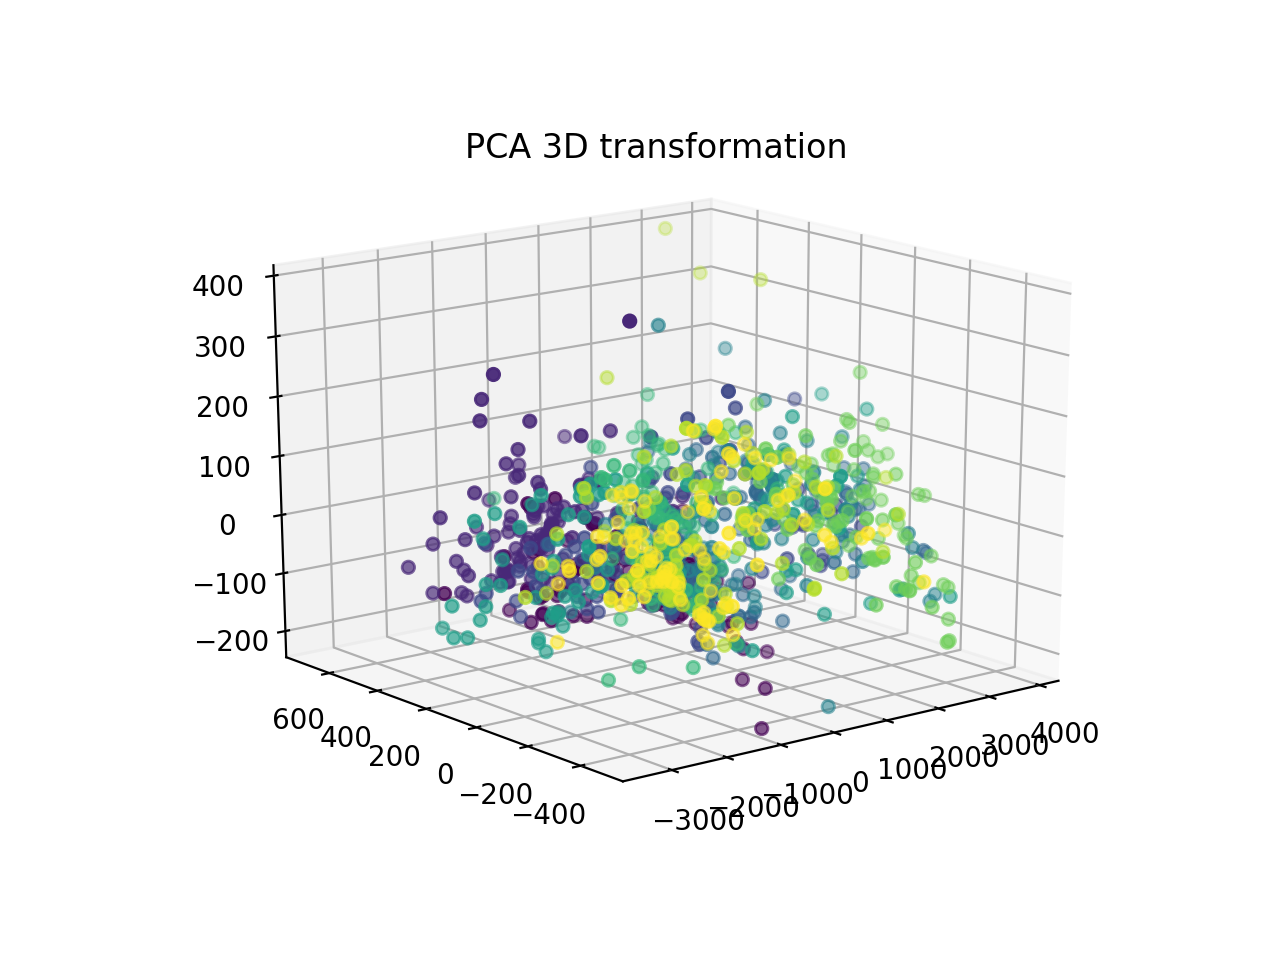
\includegraphics[width=0.45\textwidth]{pca0} 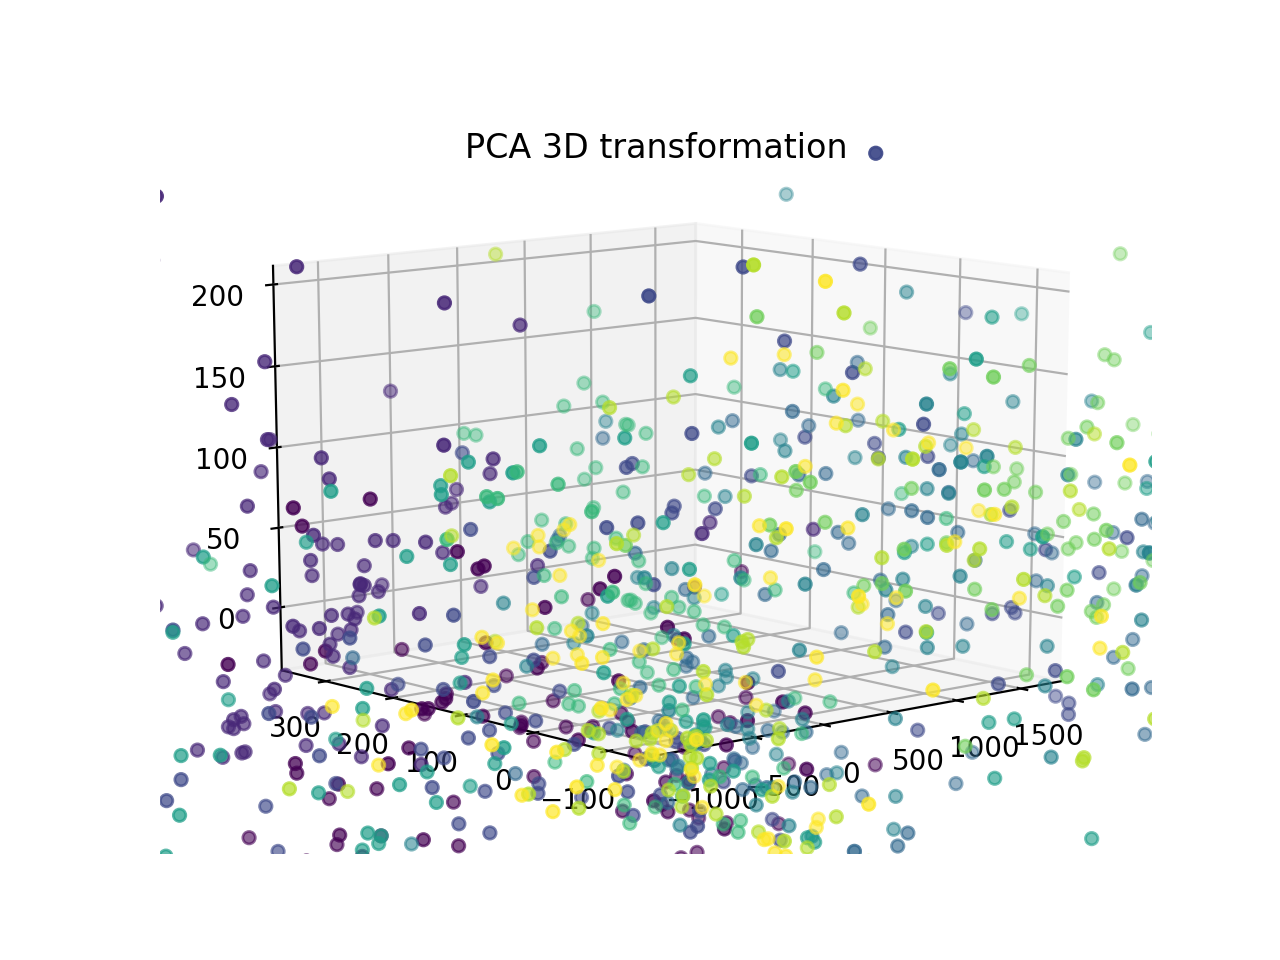
\includegraphics[width=0.5\textwidth]{pca1}
    \\ The graph on the right is a zoomed in version of the left graph. It is clear that there are many data points mixed together and the dataset is at least not linearly separable in 3 dimensions.
    \item Linear Regression: I one-hot-encoded the labels and tried to fit a linear regression. The testing and training accuracy was 0.26 and 0.31 respectively. This serves as more evidence that the dataset is non-trivial.
\end{itemize}
After these additional experiements, I am somewhat confident that my \textbf{dataset is non-trivial}. I will solidify my claim after I train my classifiers in \hyperref[notrivial]{Section 3.4}

\subsection{Performance Metrics}
I will be scoring each classfier using cross validation on the testing dataset to obtain k independent scores. These scores represent the accuracy at which the classifier sucessfully classified each data point. I'll be using the cross validated scores to create a confidence interval that will help in comparing the classifiers to each other.

\section{Description of Algorithms}
\subsection{Random Forests with Bagging}
A random forest consists of a large number of individual decision trees that form an ensemble. An ensemble bascially uses multiple algorithms to obtain more accurate predictions than any one individual of the ensemble. In a random forest, the ensemble is made up of relatively uncorrelated decision trees. Bagging (Bootstrap Aggregation) is a method that allows each decision tree in the random forest to randomly sample the dataset with replacement. Since decision trees are very sensitive the training data, this greatly increases the variablility of the decision trees. Here are the hyperparameters I will optimize:
\begin{itemize}
    \item n\_estimators: [100, 200, 300, 400, 500]
    \\ Number of trees in the forest. Affects the size of the random forest.
    \item max\_depth: [100, 200, 300, 400, 500]
    \\ The maximum depth of each decision tree. affects the complexity of each tree.
    \item max\_features: ['sqrt', 'log2', None]
    \\ The max size of the random subsets of features to consider when splitting a node.
\end{itemize}

\subsection{Support Vector Machines with a non-linear kernel}
SVMs attempts to separate datapoints by its labels by finding the best hyperplane using the large margin principle. For non-linear data, it can use the kernel trick to map the data to a higher dimension in hopes of finding a more suitable hyperplane. However, SVMs are inherently binary classifiers so it is not suitable for my dataset that has 10 unique labels. I will be using the \textbf{one-versus-all} classification technique to train my multiclass SVM. Here are the hyperparameters I will optimize:
\begin{itemize}
    \item C: [1.e-02, 1.e-01, 1.e+00, 1.e+01, 1.e+02, 1.e+03, 1.e+04]
    \\ Regularization paramenter represents how much I want to avoid misclassifying each training example. Large C will choose the a plane that correctly classifies the most training examples. Small C will choose a plane with a larger margin even if that plane wrongly classifies more training examples
    \item kernel: ['poly', 'rbf', 'sigmoid'] 
    \\ The kernel type to use when mapping the data to a new dimension space. This will affect the separablility of the data after it is mapped to a new dimension.
    \item gamma: [1.e-03, 1.e-02, 1.e-01, 1.e+00, 1.e+01, 1.e+02, 1.e+03]
    \\ Kernel coefficient for rbf, poly, and sigmoid.
\end{itemize}

\subsection{Neural Network}
A neural net is basically a bunch of algorithms, designed and modeled loosely like a human brain, that can \textbf{recognize patterns}. They all start with an input layer, which can be thought of an array of inputs such as numbers, rgb values, words, etc. The input layer is \textbf{densely connected} to the first hidden layer and the first hidden layer to the next hidden layer. There can be many hidden layers and each layer is made up of some amount of neurons. Each neuron's job is to compute a \textbf{weighted average} of its input, and this sum is passed through a non-linear activation function such as a sigmoid or ReLU. Eventually the last hidden layer will connect to an output layer responsible for outputting the prediction. The entire neural net is trained using a technique called \textbf{back propagation}, which calculates a gradient descent to nudge the weights for a perceptron towards its theoretical optimal value. Here are the hyperparameters I will optimize for my nerual net:
\begin{itemize}
    \item hidden\_layer\_sizes: [ (10, 10, 10), (20, 20, 20), (10, 10), (20, 20) ]
    \\ A tuple of length (number of layers - 2) where the element at position i represents the number of neurons in hidden layer i.
    \item activation: ['identity', 'logistic', 'tanh', 'relu']
    \\ The activation function for the hidden layer.
    \item solver: ['lbfgs', 'sgd', 'adam']
    \\ The solver for weight optimization for each neuron
    \item apha: [0.0001, 0.001]
    \\ The L2 regularization penalty parameter. This penalizes larger weight values to favor smaller values in the weight matrix. This in turn decreases the effect of the activation function, resulting in a less complex function. We want a less complex function to avoid overfitting
    \item learning\_rate\_init: [0.01, 0.001]
    \\ For my purposes, this will be the learning rate for the entirety of the training because I will be using a constant learning rate for all trials to limit the complexity of this GridSearch.
    \item max\_iter: [500, 1000] $\rightarrow$ [2000, 3000]
    \\ The limit on the number of iterations of training. The solver iterates until convergence or when it has reach the max number of iterations.
\end{itemize}

\section{Tuning Hyperparameters}
\label{tuning}
I will be using \textbf{Nested k-Folds Cross Validation} for hyperparameter tuning. In Nested k-Folds Cross Validation, I will split data randomly into two halves, X and Y. Then I will perform k-Folds Cross Validation on X to tune for optimal hyperparameters. I'll be using sklearn's \textbf{GridSearchCV} for hyperparameter tuning. Then I will take the hyper parameters tuned from X and score it using k-folds cross validation on Y. Then I will switch X and Y and repeat the process. I chose k=10 because my data has 10 different labels and this will give me 20 data points to calculate a confidence interval from. Here is a short step by step guide to my process:
\begin{enumerate}
    \item Split dataset into X and Y
    \item 10 folds cross validation on X and tune hyperparameters
    \item Use hyperparameters from 2. to create classfier C
    \item Split Y into 10 folds. For each fold i: train C on all other folds and score on current fold i. This gives 10 scores
    \item Switch X and Y and repeat steps 1 to 4. This gives 20 scores in total
    \item Use the 20 scores to calculate confidence interval for the classifier
\end{enumerate}
\subsection{Tuning Random Forests}
Here is the set of hyperparameters that I tuned for Random Forests:
\begin{itemize}
    \item n\_estimators: [100, 200, 300, 400, 500]
    \item max\_depth: [100, 200, 300, 400, 500]
    \item max\_features: ['sqrt', 'log2', None]
\end{itemize}
Each GridSearchCV on a split half the size of the data with these hyperparameters took about 184 seconds so the whole experiement took \textbf{368s} to run. \\
Let us analyze this first batch of graphs where the x-axis is max\_depth, the y-axis is mean\_test\_score, and the colors correspond to max\_features: \\
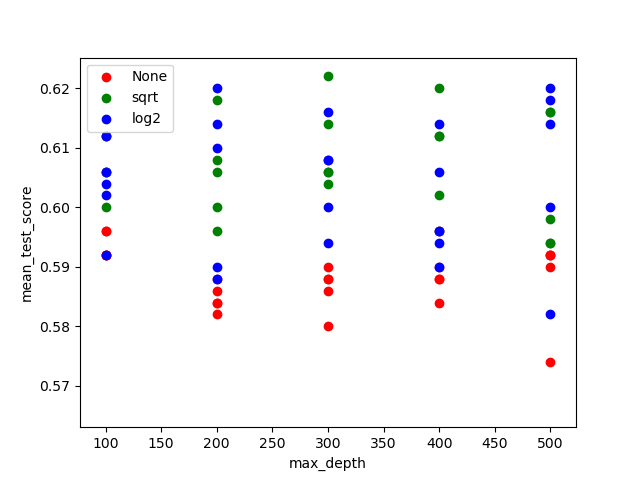
\includegraphics[width=0.5\textwidth]{RF_max_depth0.png}
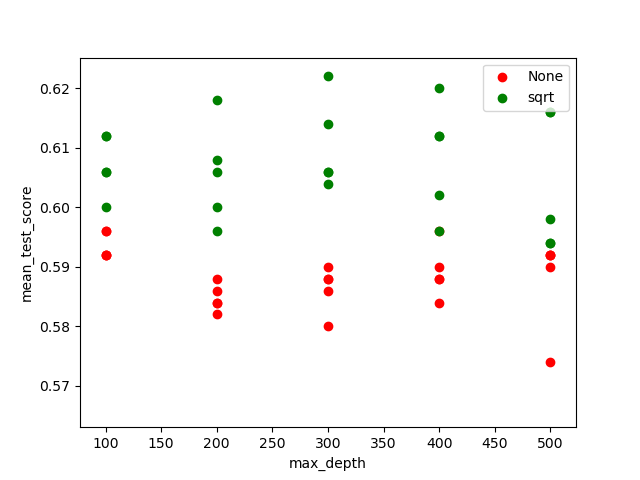
\includegraphics[width=0.5\textwidth]{RF_max_depth1.png}
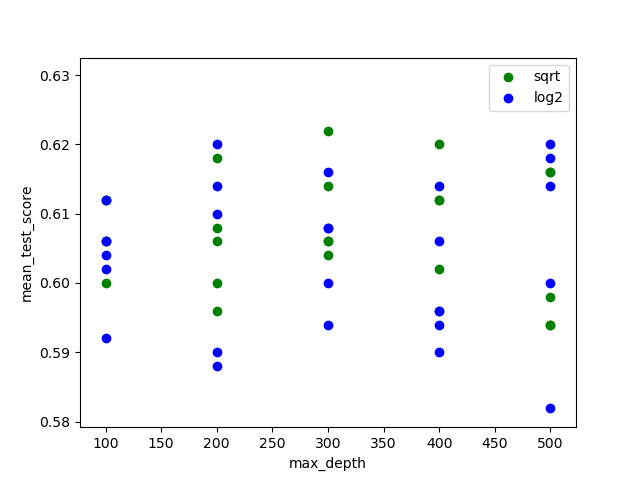
\includegraphics[width=0.5\textwidth]{RF_max_depth2.png}
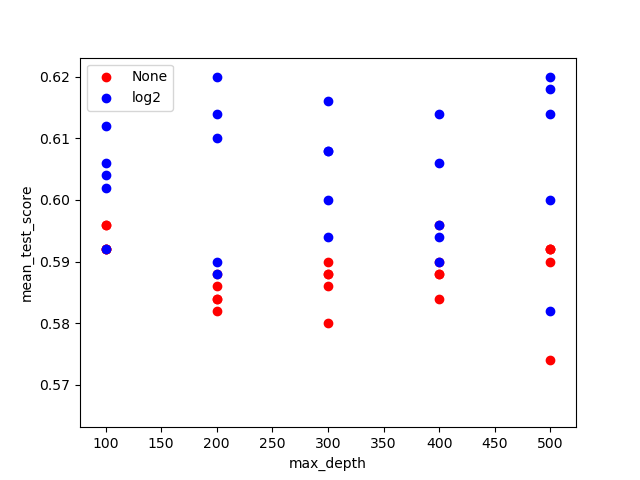
\includegraphics[width=0.5\textwidth]{RF_max_depth3.png}
Looking at these graphs, we can see that green and blue points consistently out-perform the red points. When we compare green and blue, it seems that both are evenly distributed. Both colors tend to have higher scores around 300 max\_depth. \\ \\
Let us look at the second batch of graphs where the x-axis is n\_estimators, the y-axis is mean\_test\_score, and the colors correspond to max\_features: \\
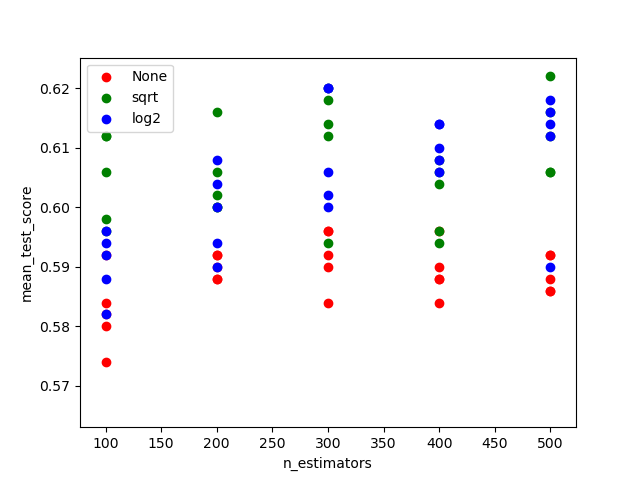
\includegraphics[width=0.5\textwidth]{RF_n_estimators0.png}
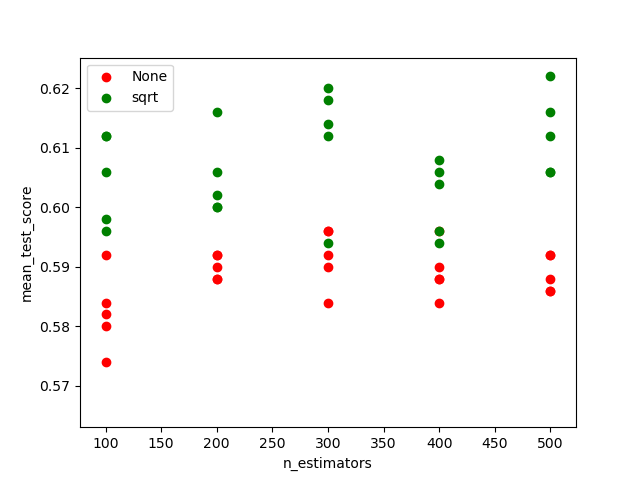
\includegraphics[width=0.5\textwidth]{RF_n_estimators1.png}
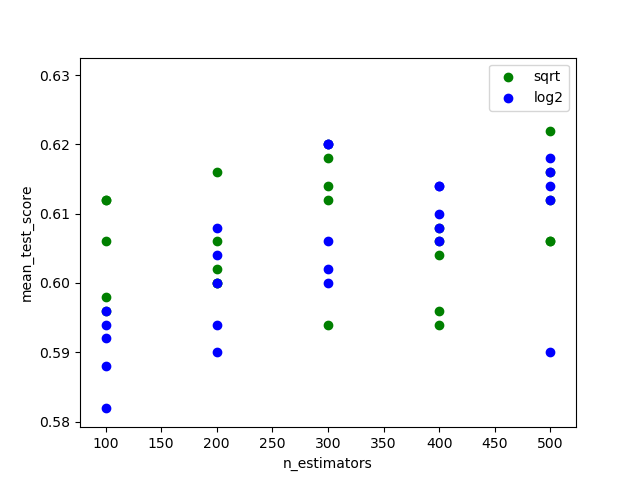
\includegraphics[width=0.5\textwidth]{RF_n_estimators2.png}
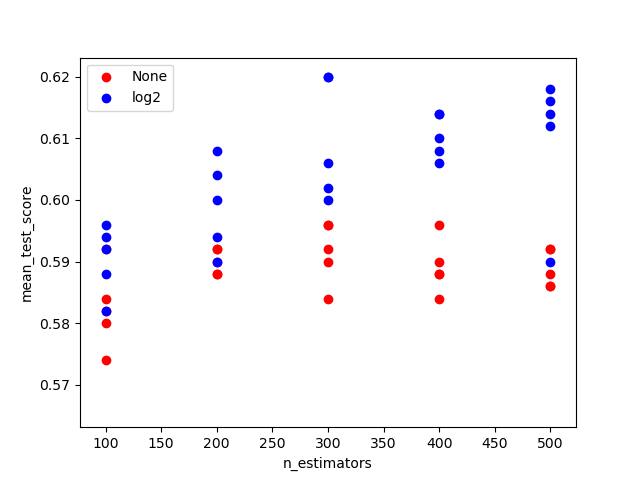
\includegraphics[width=0.5\textwidth]{RF_n_estimators3.png}
Looking at these graphs, we see again that the green and blue points out-perform the red points. The blue and green points also seem to be evenly matched as well. The blue point with the best score has around 300 n\_estimators but there seems to be an upward trend in score as n\_estimators increase for blue points. The green point with the highest score has around 500 n\_estimators. The distribution of green points does not have any noticeable trend. To further explore the relationship, I averaged the score at each x-value for the past two sets of graphs and plotted a line graph to show the trend. The shades of color are 1 standard deviation ranges of the mean for that average datapoint: \\
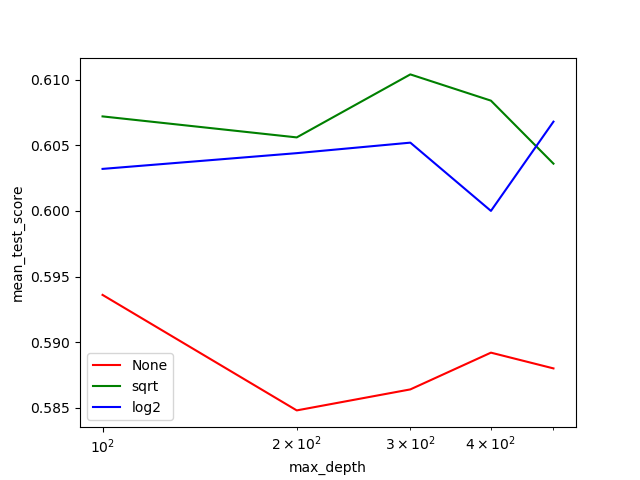
\includegraphics[width=0.5\textwidth]{RF_max_depth_line.png}
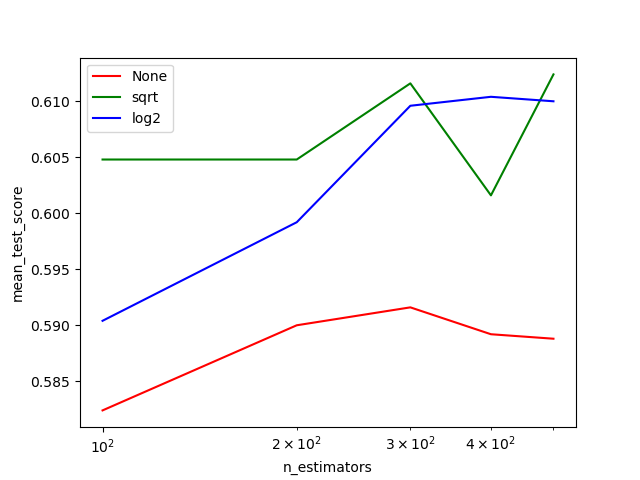
\includegraphics[width=0.5\textwidth]{RF_n_estimators_line.png}
\\
Looking at the new line graphs, it seems that the sqrt (of the number of total features) perfoms the best among the other max\_features options. Based on the graphs I would choose sqrt for the max\_features, 300 for max\_depth, and 500 for n\_estimators. The best set of hyperparameters that GridSearchCV returned was also ['max\_depth': 300, 'max\_features': 'sqrt', 'n\_estimators': 500]. This estimator had an average cross evaluated score on the testing data of around 0.595 for my run.

\subsection{Tuning Non-Linear SVMs}
Here is the set of hyperparameters that I tuned for Non-Linear SVMs:
\begin{itemize}
    \item C: [1.e-02, 1.e-01, 1.e+00, 1.e+01, 1.e+02, 1.e+03, 1.e+04]
    \item kernel: ['poly', 'rbf', 'sigmoid'] 
    \item gamma: [1.e-03, 1.e-02, 1.e-01, 1.e+00, 1.e+01, 1.e+02, 1.e+03]
\end{itemize}
Each GridSearchCV on a split half the size of the data usually took 7 seconds to run. However, sometimes it would take significantly longer to converge. My results took \textbf{14s} to complete. Here are the graphs of mean\_test\_score versus C and gamma for each kernel: \\
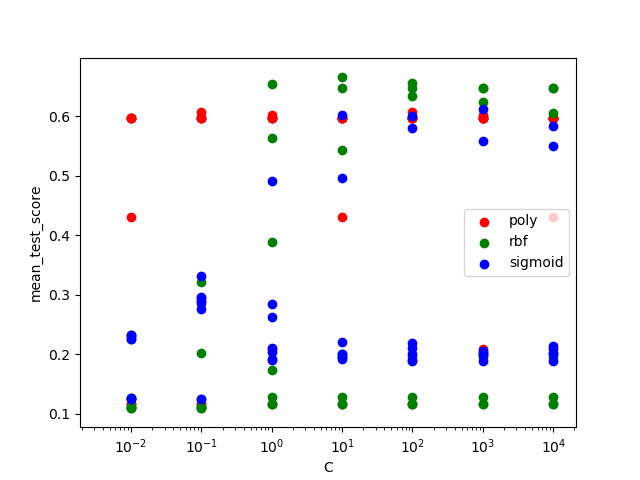
\includegraphics[width=0.5\textwidth]{SVM_C0.png}
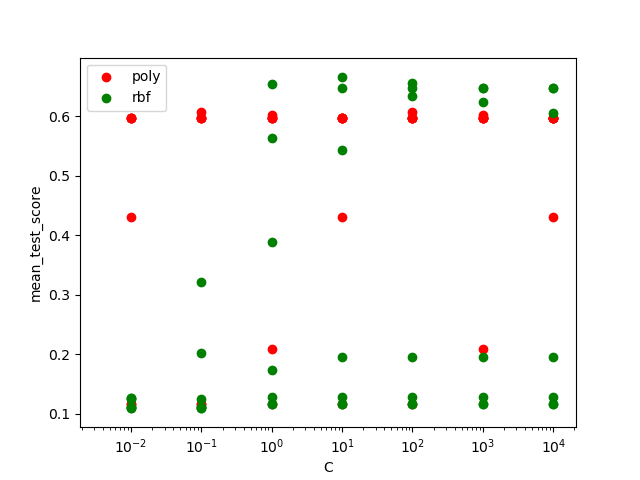
\includegraphics[width=0.5\textwidth]{SVM_C1.png}
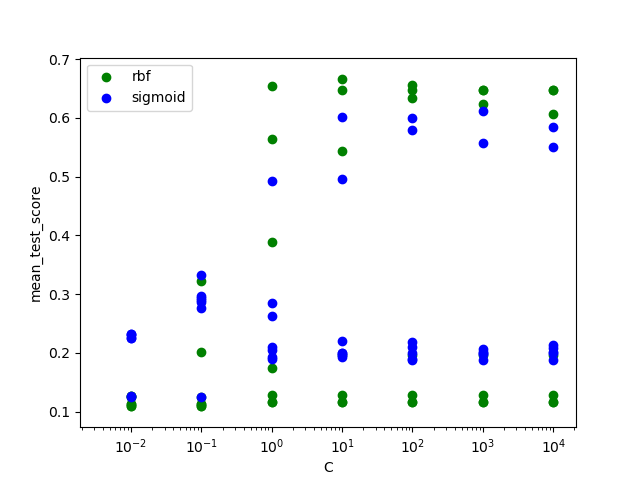
\includegraphics[width=0.5\textwidth]{SVM_C2.png}
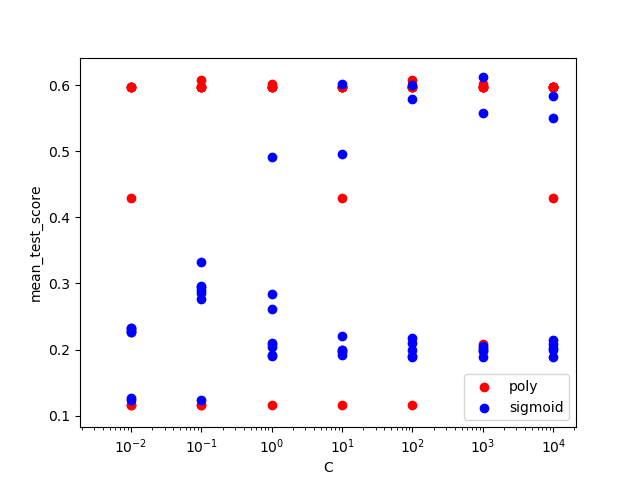
\includegraphics[width=0.5\textwidth]{SVM_C3.png}
For the graphs with C on the x-axis, we see that rbf has the best performing individuals but it also has the lowest performing individuals. The individuals in poly seem to score better than the individual of sigmoid. I think it's interesting to note that the highest performing individuals of rbf have C values of 1 or more. This means that the classifier will try to correctly classify as many training examples as possible and be more likely to overfit. However in our case, a larger C value actually produced better results.
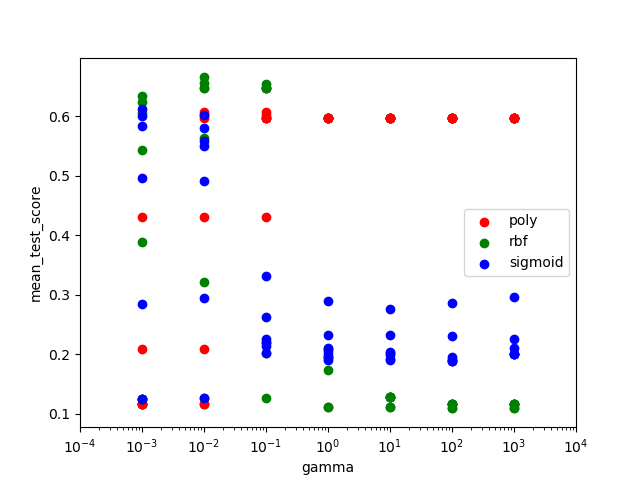
\includegraphics[width=0.5\textwidth]{SVM_gamma0.png}
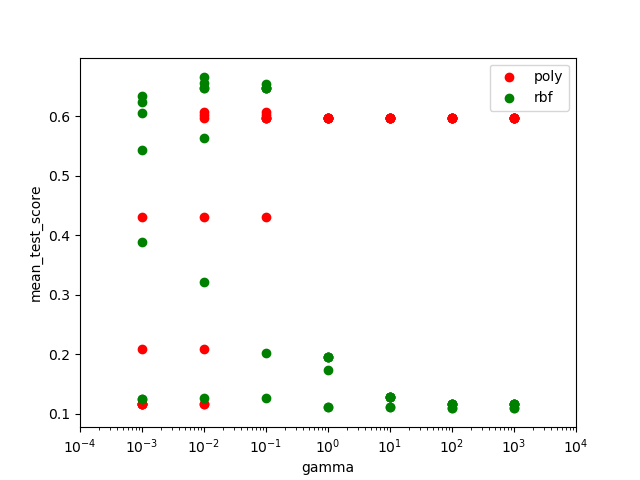
\includegraphics[width=0.5\textwidth]{SVM_gamma1.png}
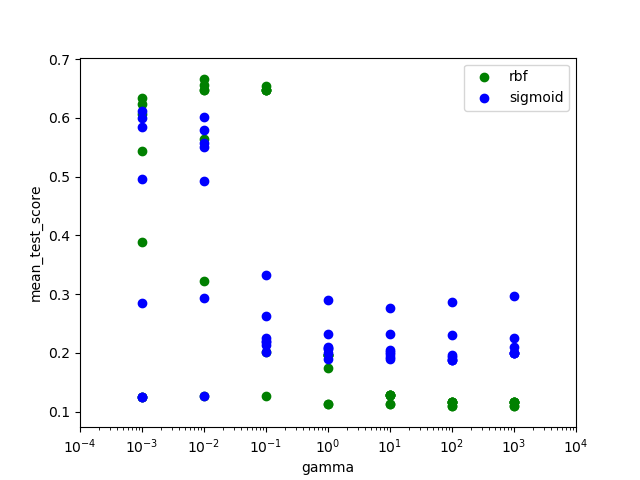
\includegraphics[width=0.5\textwidth]{SVM_gamma2.png}
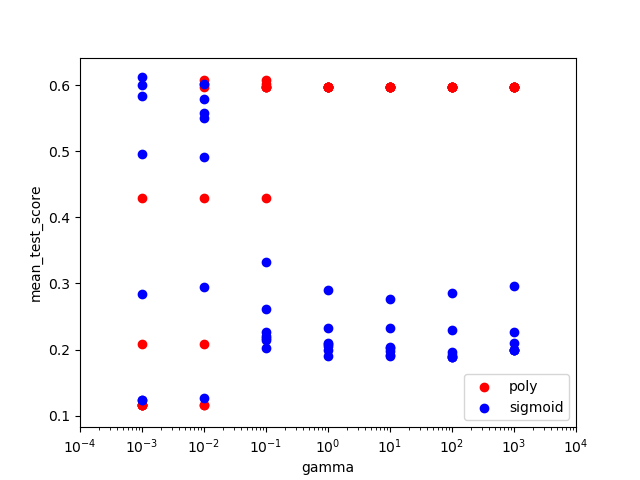
\includegraphics[width=0.5\textwidth]{SVM_gamma3.png}
We see a bit more pattern for the graphs with gamma on the x-axis. All of rbf's highest scoring individuals have a gamma of 0.1 or lower while poly's highest scoring individuals have a gamma of 0.01 or higher. This is because the kernel coefficient, gamma, has different optimal values for different kernels. \\
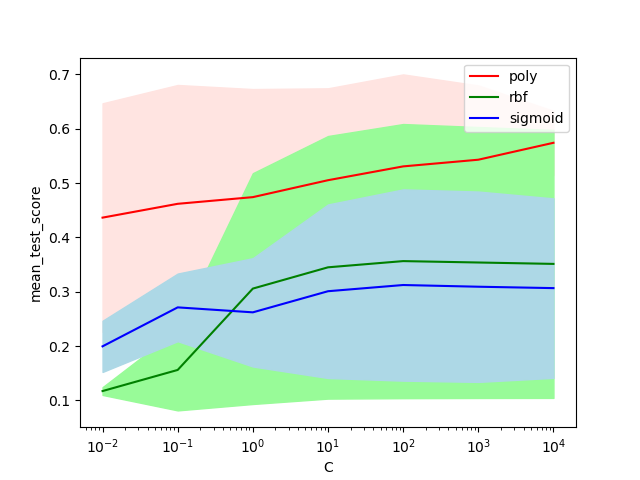
\includegraphics[width=0.5\textwidth]{SVM_C_line.png}
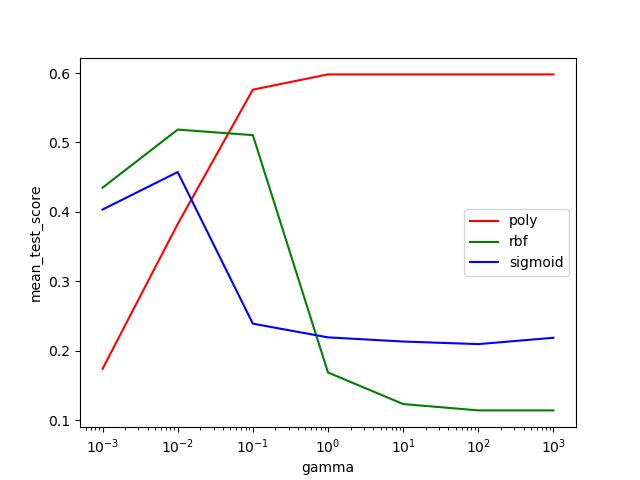
\includegraphics[width=0.5\textwidth]{SVM_gamma_line.png}
Looking at the average scores for C and gamma values, we actually see some contradicting results. From the previous graphs, it looked like rbf would be the best choice for highest performing indviduals. In terms of consistency and average scores, though, poly performs a lot better than the other two kernels. Note that the standard deviation for the gamma graph decreases due a smaller number of datapoints, not because of an increase in consistency. Based on the averages, I would choose poly because its average score is better than the other kernels. I would choose C=10000 and gamma = 100. The best estimator from GridSearchCV was rbf simply due to it having the highest scoring individual. 
\subsection{Tuning Neural Nets}
Here is the set of hyperparameters that I tuned for MLP:
\begin{itemize}
    \item hidden\_layer\_sizes: [ (10, 10, 10), (20, 20, 20), (10, 10), (20, 20) ]
    \item activation: ['logistic', 'relu']
    \item apha: [0.0001, 0.001]
    \item learning\_rate\_init: [0.01, 0.001]
    \item max\_iter: [500, 1000] $\rightarrow$ [2000, 3000]
    \\ None of my MLPs would converge within 1000 iterations so I increased the max\_iter
\end{itemize}
Each GridSearchCV on a split half the size of the data took 950 - 1000 seconds to run. This first round of my experiment took \textbf{2008s} to complete. \\
These combinations of hyperparameters took a long time to run but did not give me too much data. Here are some graphs showing the effects of each hyperparameter: \\
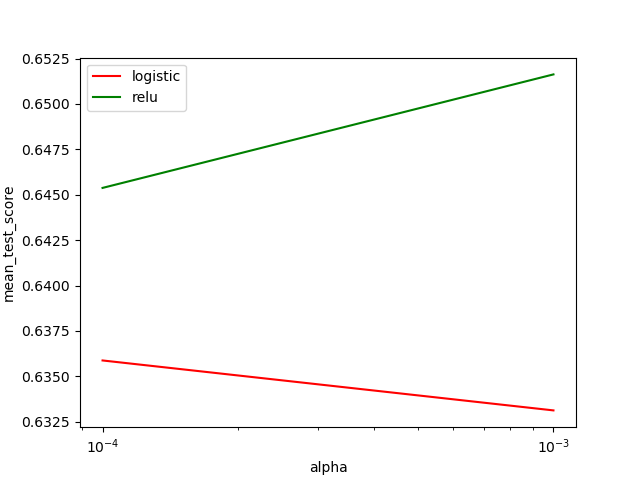
\includegraphics[width=0.33\textwidth]{MLP_alpha_line.png}
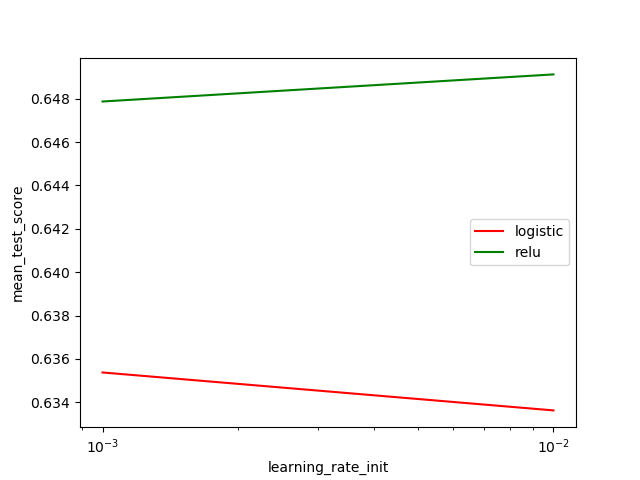
\includegraphics[width=0.33\textwidth]{MLP_learning_rate_init_line.png}
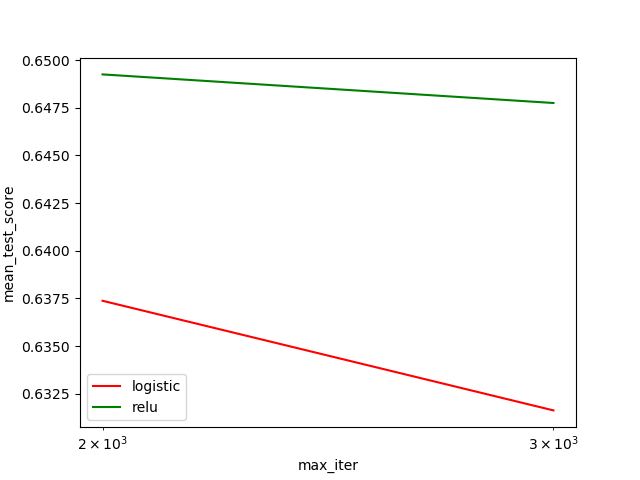
\includegraphics[width=0.33\textwidth]{MLP_max_iter_line.png}
Each graph was made this way: I took the average mean\_test\_score of each activation function at each x-value of (alpha, learning\_rate\_init, max\_iter). Since I only had two different values for each of these, there is a straight line connecting the two averages to show a very rough estimate of a trend. From these graphs, we can see that higher scores are associated with:
\begin{itemize}
    \item higher alpha value
    \item higher learning rate for relu, lower for logistic
    \item lower max iterations. This is probably because a higher alpha reduces \textbf{overfitting}
\end{itemize}
Looking at the MLP\_out.txt, I printed the best params of the two grid searches I did. I noticed that 3 hidden layers did better with a higher learning rate while 2 hidden layers did better with a lower learning rate. From these results, it is clear that using relu activation for the neurons performed a lot better than using logistic. This makes sense because the logistic function Sklearn's MLP uses is the sigmoid function. The sigmoid function is good for binary classification but relu is used in almost every other type of problem. It is hard to conclude anything about the learning rate and it seems we do better with lower max\_iterations. So I took these results to run another experiment in which I only vary alpha and learning rate. Here are the hyperparameters:
\begin{itemize}
    \item hidden\_layer\_sizes: [(100, 100, 100)]
    \item activation: ['relu']
    \item apha: [0.0001, 0.0005, 0.001, 0.005, 0.01, 0.05, 0.1]
    \item learning\_rate\_init: [0.001, 0.005, 0.01, 0.05, 0.1]
    \item max\_iter: 1500
\end{itemize}
This experiment took \textbf{100s}. Here are the resulting graphs. \\
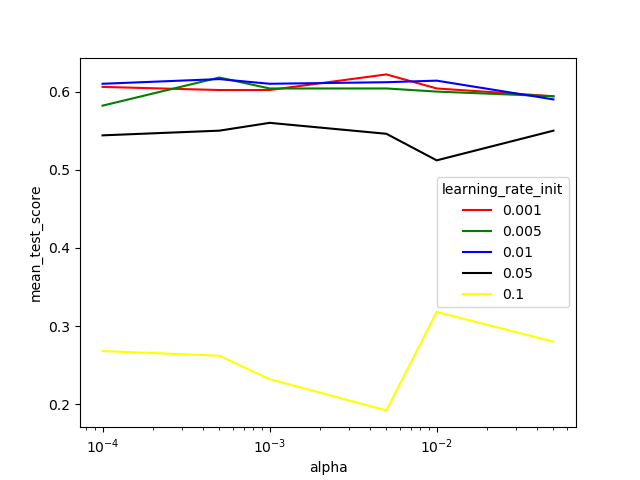
\includegraphics[width=0.5\textwidth]{MLP_fin_alpha_line.png}
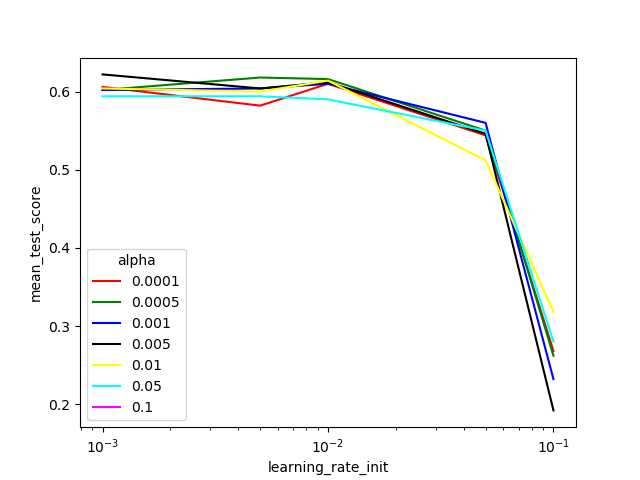
\includegraphics[width=0.5\textwidth]{MLP_fin_learning_rate_init_line.png}
From the left graph, we can see that too high of a learning rate is obviously bad. There is not much difference the learning rates less than 0.05 when alpha is varied. From the right graph, we can see again that if learning rate is too big, the score will drop drastically. This is expected as a high learning rate can cause a model to diverge instead of converging. The best individuals from both GridSearchCVs had a learning\_rate\_init of 0.001 and alpha of 0.005. At this point, I manually zoomed into the lines at the top in the left graph. \\ 
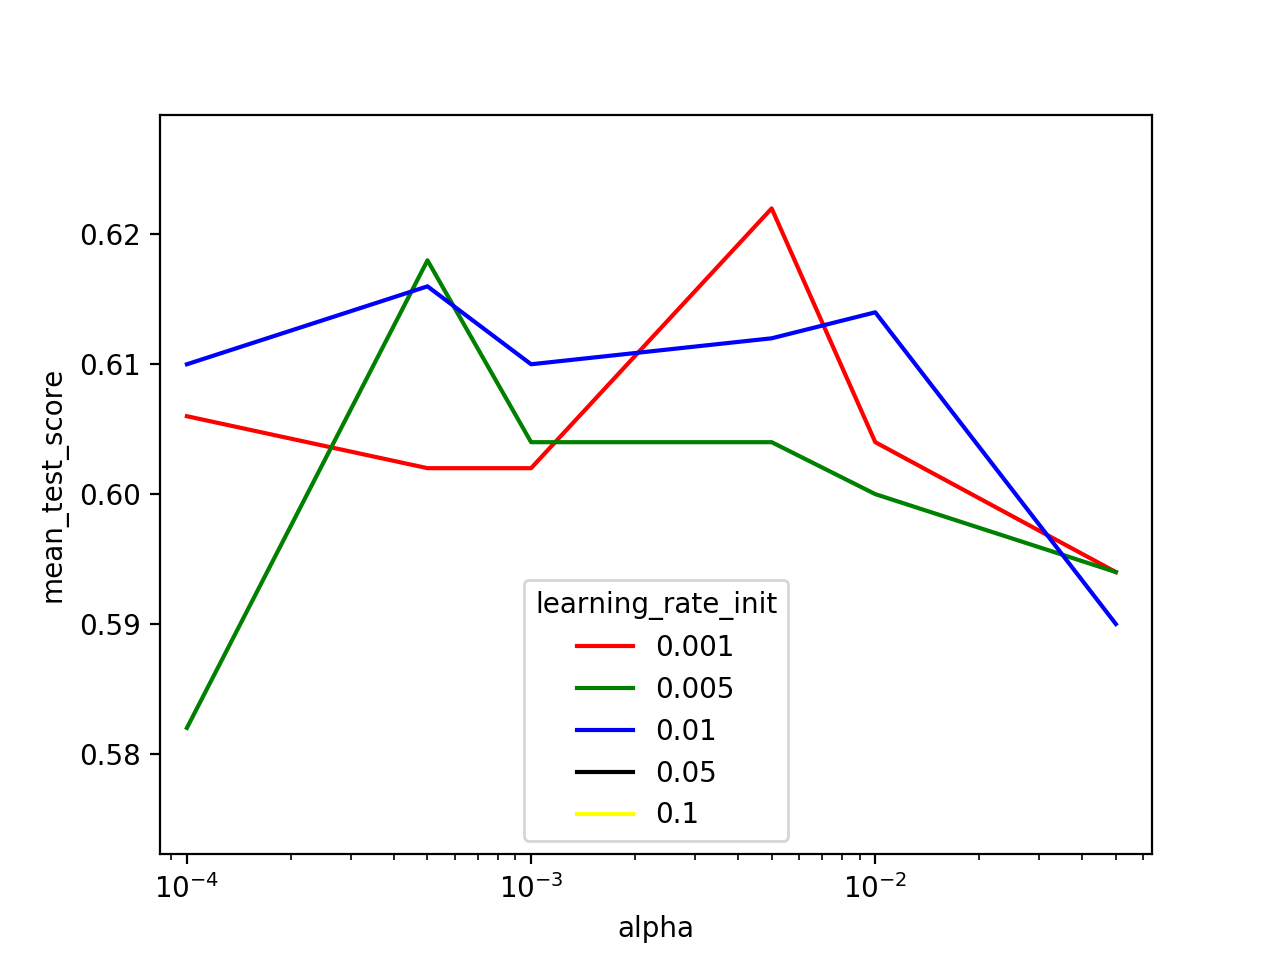
\includegraphics[width=0.75\textwidth]{MLP_fin_alpha_line_zoom.png} \\
With a closer look, we can tell that for each learning\_rate\_init, there is an optimal alpha associated with it. The hyperparameters I would choose to train for this dataset is relu activation, -0.005 alpha, (100, 100, 100) hidden layers, 0.001 learning rate and 1500 max iterations.
\subsection{Non-Triviality}
\label{notrivial}
In addition to my initial tests (\hyperref[trivial]{Section 1.2}) to determine if my dataset was trivial, the performance and variability that is shown these three classifiers further solidify my claim that my dataset is non-trivial.

\section{Comparing Algorithm Performance}
The metrics I used to evaluate each classifier was detailed in \hyperref[tuning]{Section 3}. With the 20 cross validated testing scores, I created a 95\% confidence interval for each classifier's performance:
\begin{itemize}
    \item RandomForest: [0.5942999477145694, 0.6077000522854301]
    \item Non-Linear SVM: [0.6097518259758751, 0.6202481740241249]
    \item MLP Neural Net: [0.607693718679951, 0.618306281320049]
\end{itemize}
Based on the confidence intervals, it seems that RandomForest was the worst performing classfier and is barely statistically significant from the other two. SVM had a larger range than the Neural Net but neither were statistically significant from each other. I chose not to look at the confusion matrix due to the nature of the dataset. Since I used one-vs-all classification, the confusion matrix would not tell me the labels that missclassifications chose. Also, since there is no need to prefer false negatives over false positives or vice versa, there is no need to look at a confusion matrix. Based off of performance \textbf{only} I would choose Non-Linear SVM because it has the highest range of confidence interval.

\section{Conclusion}
To consider all metrics, I would choose the MLP Neural Net to use in real practice because of many factors. It is the most flexible and can handle a greater variety of problems. In my experiements, MLP training and hyperparameter tuning was not the slowest even though it can be a very complex model. It took about 100 seconds to find optimal hyperparameters for learning rate and alpha for neural net. I am not factoring the other hyperparameters because a neural net can solve most problems with just one hidden layer. For RandomForest, it took 4 times as long (400s) to find optimal parameters for a model with less accuracy. I did not choose SVM due to its variablility in tuning time. Sometimes it takes 20 seconds, others it can take hours. I do not completely understand the math behind this phenomenon so I am hesitant to choose SVMs for use in real life. \\ \\
I also believe the neural net is very fitting for data on this domain because humans are who decides the genre of a piece of music. The model that most closely resembles a human brain is the neural net. However, one down fall of neural nets is that the input data must be pre-processed. I was lucky to find a dataset that was complete. But if we are dealing with sounds, all features of a piece can be calculated with its sound wave, which means you can get the data if you try hard enough. 

\subsection{Further Thoughts}
I would be very interested in exploring the algorithms of companies like Spotify that can recommend music to users based on their preferences. I'm sure that genre is a feature that is used in their algorithm. 

\nextproblem

\section{Acknowledgements}

\href{https://www.quora.com/What-are-C-and-gamma-with-regards-to-a-support-vector-machine}{Where I learned what C and Gamma are} \\
\href{https://scikit-learn.org/stable/index.html}{Sci-kit Learn} \\
\href{https://machinelearningmastery.com/save-load-machine-learning-models-python-scikit-learn/}{Pickling my Gridsearch Results} \\
\href{https://matplotlib.org/3.1.1/contents.html}{Matplotlib Docs} \\


\end{document}

